%\vspace{-3mm}
\section{Evaluation}

We test our prototype of DASF on a Galaxy Nexus (\textit{GT-I9250}).
%,which includes a 1.2 GHz dual-core ARM Cortex-A9 processor,
%1 GB of RAM, and 16 GB of flash memory. 
Our goal is to validate that DASF provides adequate protection against the
previously discussed security threats, and evaluate the performance overhead.
% and provide a
%performance evaluation for the system overhead. 

\subsection{Security Evaluation}

As previously discussed, we consider four different
types of security threats that DASF must provide protections
against. Due to the space constraint, we present our study of the
security evaluation by using the following carefully selected
attack examples which emulate the most adverse environment. 

%\textit{(1) legitimate user misbehavior},
%\textit{(2) malicious users}, \textit{(3) application misbehavior},
%and \textit{(4) malicious applications}.  
%Since CleanOS addresses
%the 2nd security threat by providing a mechanism for revoking sensitive
%data and we assumed that our model was built on top of CleanOS, we do not
%evaluate that security threat.  However, we perform the following three
%tests to show that DASF adequately addresses the remaining
%security threats.

\begin{itemize}
\item \textbf{Legitimate user misbehavior.}  We create an application
that receives data from the server that has restrictions imposed on
  the data.  Next, we attempt to manually save and forward the data by
  passing it to other applications on the device that attempt to
  perform these operations. 
\item \textbf{Malicious users.} Pretending to be a malicious user, we
  launch a device stealing attack to obtain the stored PHI.
\item \textbf{Application misbehavior.}  We create an application that requests
  data from the server (e.g., an MRI image) that is restricted to be saved
  to the device.  When the application is receiving the data, it attempts
  to break the policy by writing the data directly to a file.
\item \textbf{Malicious applications.}  We created a malicious voice memo recorder
  application that attempts to steal information from the environment. Our
  voice memo recorder requests the \textit{record audio} permission
  and the \textit{Internet} permission to allow users to sync memos to their
  other devices.  However, the voice memo recorder maliciously launches
  a background service to secretly record audio in the background and
  transmits the recorded audio to an external server.
\end{itemize}

In the first test, a scenario was created where a user was viewing an image
transmitted from the server with the write-to-flash permission disabled.  Then
the user tried to save the image (e.g., by long pressing on the image to have
the option to save it to the SD card) to the local flash storage.  This attempt
was defeated because the image's privacy tag was detected by our enforcement
hooks, and the write operaton was blocked.
%the image's privacy tag checking raised a red flag and 
%then the flash memory writing is blocked. 

%We ran the first test and found that DASF successfully blocked the
%data from being forwarded from the device and saved to the
%device. Thus, DASF enforced the policy imposed on the data from the
%server. 

The second test emulated a device theft scenario where a device is reported
missing. Given the security features deployed in DASF, it is the attacker's
best interest to immediately disconnect the device from Internet (to evade the
launching of the system counter-attack mechanism, e.g., remote wipe) with an
attempt to compromise the PHI stored in a previous session. This attack attempt
was defeated since the system forced the termination of the \textit{medical
application} after a specific number of consecutive server heartbeats (e.g.,
10) were missed, which released the memory containing the PHI.

%When we ran the third test, we confirmed that DASF
%successfully blocked the data from being saved to a file.  Moreover, we
%modified the application to check the sensitivity level on the data
%received and determine whether to store the data in a file or keep it
%in main memory.

In the third test, we developed a misbehaving application that
silently checks the received data sensitivities and stores the highly
sensitive data to a file (without the proper authorization). Again,
this attempt is defeated by the DASF's enforcement hooks. 


%To prevent malicious applications from attempting to steal sensitive
%information stored on the device (e.g., PHI information authorized to
%be saved to the device), we rely on Android's file system privileges
%(e.g., UIDs) and our restriction that medical applications are
%assigned a unique UID.
For the last test, we started the malicious
voice memo recorder and confirmed that it successfully recorded data
in the background.  Next, we created another application that
restricts the \textit{record audio} permission when the user presses a
button. DASF successfully closed the malicious voice memo recorder,
including its background service, and prevented it from being opened
again until the \textit{record audio} permission was
unrestricted. Actually, an easy extension can be designed to use RFID
tags, instead of pressing a button, to restrict the permission. So
doctors can simply wave their devices when entering areas where
conversations may include PHI data (e.g., outside of patient rooms).  

%\vspace{-3mm}
\subsection{Performance Evaluation}

Since DASF is invoked whenever an application, or application
component is started, we test the performance overhead of starting
activities and services on the Galaxy Nexus running our prototype.  To get
a baseline for comparison, we repeated the tests on the stock
Android \textit{Jellybean} platform and on TaintDroid.  Furthermore,
we also tested the overhead of \textit{medical applications} using our
message protocol. 

\textbf{Application Component Overhead.}  Whenever an activity or
service is started, our\textit{Privilege Restriction Service} is
invoked to determine whether the activity or service may be started.
Therefore, we tested the time that it takes to launch activities and
services.  We ran the tests for 10 times and record the average
value.  The same procedures were repeated on the stock
Android \textit{Jellybean} platform and on TaintDroid.  

Fig.~\ref{fig:component} shows the performance overhead of starting
activities and services on our prototype, the stock
Android \textit{Jellybean} platform, and on TaintDroid. As the figure
shows, our prototype takes 118 milliseconds on average to start an
activity and 17 milliseconds on average to start a service.  The stock
Android \textit{Jellybean} platform takes 94 milliseconds on average
to start an activity and 8 milliseconds on average to start a service.
The TaintDroid platform takes 115 milliseconds on average to start an
activity and 14 milliseconds on average to start a service.  We assume
that the overhead when comparing TaintDroid and the stock
Android \textit{Jellybean} platform is due to the extra memory
allocated for the privacy tags in the Java stack. 
Compared to TaintDroid, our prototype results in
a minimal overhead on starting activities and services. 

\begin{figure}[ht]
\centering
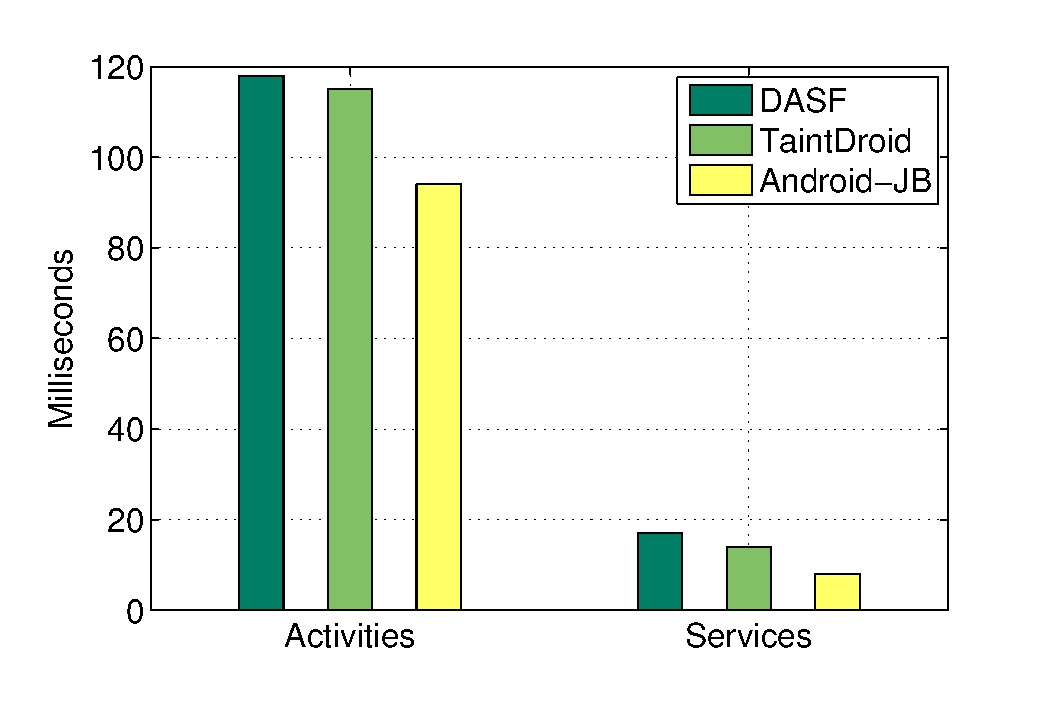
\psfig{file=performance1.eps, width=2.5in}
\caption{Performance overhead when starting activities and services}
\label{fig:component}
\end{figure}

\textbf{Message Protocol Overhead.}  To test the overhead of our
message protocol, we create an application that requests data of
varying lengths from the server. The data lengths are 1-KB, 5-KB,
100-KB, 1-MB, 5-MB, and 50-MB. We record the time that it takes
the \textit{MessageInputStream} to receive the message and pass the
data back to the application.  We disregard the time that it takes to
transmit the data over the network since that is related 
to the overhead of the network speed rather than the overhead caused by
our message protocol.  

Further, we also record the time that it takes the system to
enforce policy \textit{restrictions} and \textit{unrestrictions}.  As
Fig.~\ref{fig:performance} suggests, our message 
protocol spends 54.9 microseconds on average to parse and returns 1-KB of
data back to the application, 73.2 microseconds on average for 5-KB, 
720.2 microseconds on average for 100-KB, 8 milliseconds on average
for 1-MB, 49 milliseconds on average for 5-MB, and 468 milliseconds
on average for 50-MB.  Furthermore, it takes 81 milliseconds on average
to impose permission restrictions and around 2 milliseconds on average
for permission unrestrictions.

\begin{figure}[ht]
\centering
\subfigure[Data Message Overhead]{
	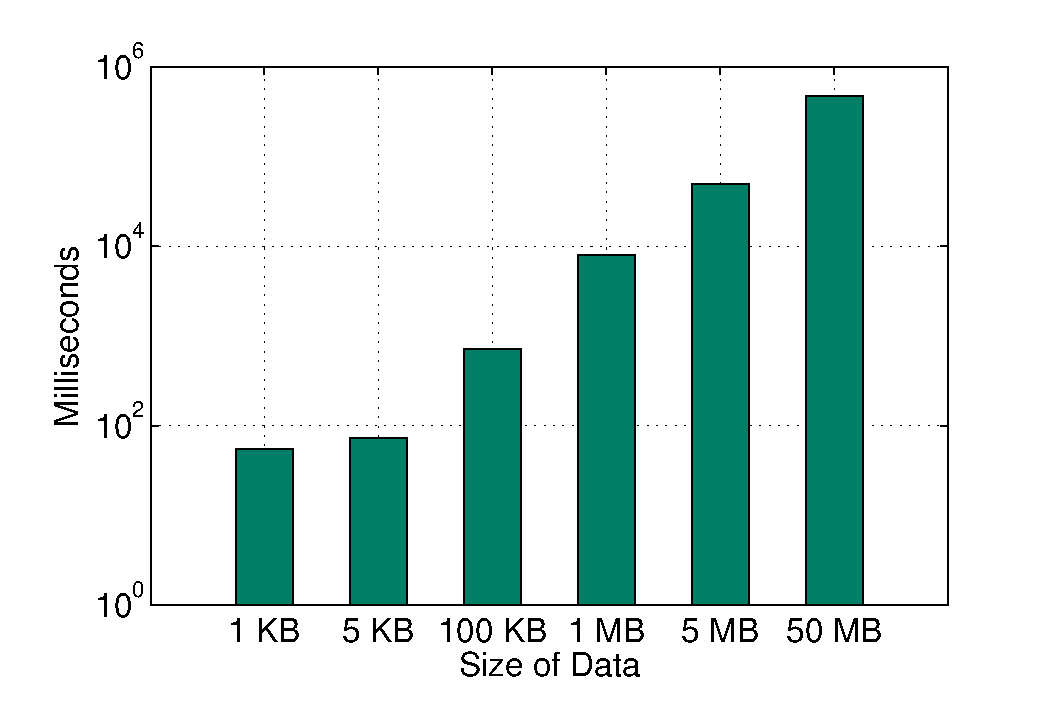
\psfig{file=performance2.eps, width=2.5in}
	\label{fig:kbperformance}
}
\subfigure[Privilege Control Message Overhead]{
	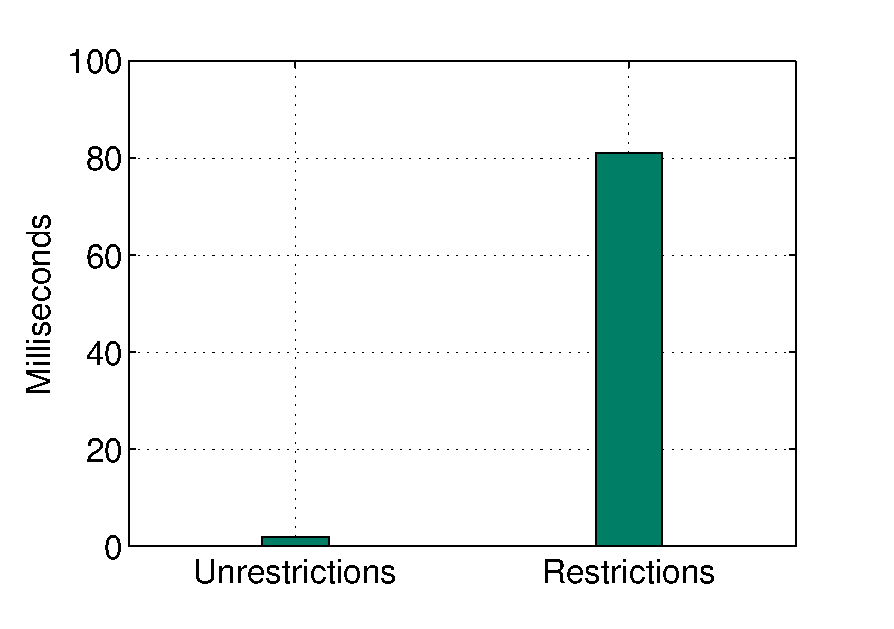
\psfig{file=performance3.eps, width=2.5in}
	\label{fig:policyperformance}
}
\caption{Message Protocol Performance Overhead}
\label{fig:performance}
\end{figure}

\subsection{Limitations and Future Work}

%There are three current limitations of the DASF prototype.  First,
%the sensitivity level of the data can be cleared since TaintDroid's
%taint propagation logic does not address implicit flows. This is a major
%concern because applications can clear the sensitivity
%level from data and break the security policies imposed on that data.
%Second, TaintDroid also does not allow applications to use third-party
%native libraries since they can be used to clear privacy tags.  Third,
%DASF does not currently handle propagating
%the sensitivity level of data displayed on the screen.  Therefore,
%a user can take a picture, from a separate camera, on the device
%screen and, as the result, acquires the picture that is unauthorized. 

There are mainly four limitations of the DASF prototype.  First, 
the privacy tags of the data collected by applications can be cleared since
TaintDroid's propagation logic does not address implicit flows. As a result,
applications may subvert the security policies imposed on that data.  As future
work, we will address this problem by integrating SpanDex's\cite{cgl+14}
technique of propagating privacy tags through implicit flows.  Second, DASF
does not allow applications to use third-party native libraries (due to
TaintDroid's restrictions), since TaintDroid cannot track information flows
through native code. This limitation can be addressed by assigning privacy tags
to the entire process and using process-level enforcement once the JNI boundary
has been crossed, and enforcing the communication protocol to incur in the
kernel.  Third, DASF does not currently handle propagating the sensitivity
level of data displayed on the screen. Therefore, a user can take a screenshot
to save or export data displayed on the screen. We leave it as future work to
propagate privacy tags from data used during the rendering of the user
interface to Android's SurfaceFlinger component. Fourth, DASF may undesirably
evict data in RAM during short network disconnects. Therefore, as future work,
we aim to develop a mechanism to tolerate short network disconnects without
sacrificing the security countermeasure capabilities of DASF.


%An immediate solution would introduce the
%application authentication procedure to certify the authenticity of the
%applications. A permanent fix is to get rid of TaintDroid and address
%the problem in the native Android. 
%Second, DASF does not
%allow applications to use third-party native libraries (due to
%TaintDroid's restrictions), since they can be used to clear privacy
%tags.  Our future work will address the above two limitations by
%directly building our DASF on the native Android. Third, DASF does not
%Therefore, a user can take a picture, from a separate
%camera, on the device screen and, as the result, acquires the picture
%that is unauthorized.  At this moment, we have no solution to address 
%this type of privacy breaches but argue that the amount of the
%information leakage is limited because the quality of the image
%captured in the above way (e.g., the number pixels per inch) has no
%comparison to the original quality.


%Our future work includes the system enhancement in the following aspects.
%First, we need to develop a mechanism to differentiate the network brokeage and
%security attacks.  Ideally, DASF will allow a short disconnect operation
%without sacrificing the security countermeasure capabilities. Second, we will
%start our development of DASF on a native Android system instead of the
%TaintDroid to further improve the system latency performance and enhance the
%security performance as discussed previously.  





